\documentclass[a4paper,12pt]{article}
\usepackage{cmap}
\usepackage[T2A]{fontenc}
\usepackage[utf8]{inputenc}
\usepackage[english,russian]{babel}
\usepackage{listings}
\usepackage{amsmath}
\usepackage{float}
\usepackage{csquotes}
\usepackage{graphicx}
\usepackage{xcolor}
\usepackage{hyperref}
\usepackage{mathtools}

\renewcommand{\theequation}{\thesection.\arabic{equation}}


\author{Шерепа Никита}
\title{ThinkDSP. Лабораторная 3. Апериодические сигналы.}
\date{\today}

\graphicspath{{res/screenshots}}

\begin{document}%
	
	\maketitle
	
	\newpage \tableofcontents
	\newpage \listoffigures
	\newpage \lstlistoflistings
	
	\newpage
	
	\definecolor{dkgreen}{rgb}{0,0.6,0}
	\definecolor{gray}{rgb}{0.5,0.5,0.5}
	\definecolor{mauve}{rgb}{0.58,0,0.82}
	
	\lstset{
		language=Python,                 % выбор ЯП для подсветки 
		basicstyle=\small\sffamily, % размер и начертание шрифта для подсветки кода
		numbers=left,               % где поставить нумерацию строк (слева\справа)
		numberstyle=\tiny,           % размер шрифта для номеров строк
		stepnumber=1,                   % размер шага между двумя номерами строк
		numbersep=5pt,                % как далеко отстоят номера строк от подсвечиваемого кода
		aboveskip=3mm,
		belowskip=3mm,
		showstringspaces=false,
		columns=flexible,
		captionpos=b, 
		basicstyle={\small\ttfamily},
		numbers=left,
		numberstyle=\tiny\color{gray},
		keywordstyle=\color{blue},
		commentstyle=\color{mauve},
		stringstyle=\color{dkgreen},
		breaklines=true,
		breakatwhitespace=true,
		tabsize=3
	}
	
	\section{Упражнение 3.1}
	
	\begin{enumerate}
		
		\item \textbf{Задание}
		
		Запустите и прослушайте примеры из блокнота \textit{chap03.ipynb}.
		В примере с утечкой замените окно Хэмминга одним из окон, предоставляемых \textit{NumPy}, и посмотрите, как они влияют на утечку.
		
		
		\item \textbf{Ход работы}
		
		Для начала создадим утечку
		\begin{lstlisting}[caption=Пример утечки]
			from thinkdsp import decorate
			from thinkdsp import SinSignal
			
			signal = SinSignal(freq=440)
			duration = signal.period * 30.25
			wave = signal.make_wave(duration)
			spectrum = wave.make_spectrum()
			
			spectrum.plot(high=880)
			decorate(xlabel='Frequency (Hz)')
		\end{lstlisting}
		
		\begin{figure}[H]
			\centering
			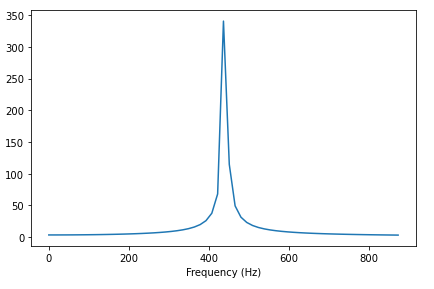
\includegraphics[width=0.75\textwidth]{1_1.png}
			\caption{Визуализация утечки}
			\label{fig:1.1}
		\end{figure}
		
		Теперь заменим окно Хэмминга на другие 4 окна из \textit{NumPy}
		\begin{lstlisting}[caption=Создание 4х новых окон]
			import numpy as np
			for window_func in [np.bartlett, np.blackman, np.hamming, np.hanning]:
			wave = signal.make_wave(duration)
			wave.ys *= window_func(len(wave.ys))
			
			spectrum = wave.make_spectrum()
			spectrum.plot(high=880, label=window_func.__name__)
			
			decorate(xlabel='Frequency (Hz)')
		\end{lstlisting}
		\begin{figure}[H]
			\centering
			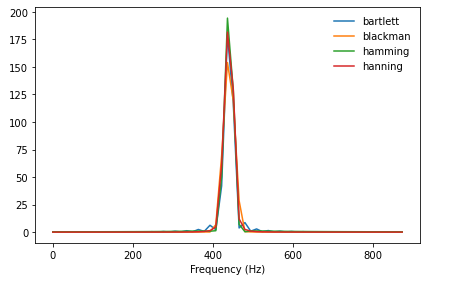
\includegraphics[width=0.75\textwidth]{1_2.png}
			\caption{Сравнение 4х новых окон с окном Хэмминга}
			\label{fig:1.2}
		\end{figure}
		Из графика видно, что все 4 окна успешно справляются с уменьшением утечки.
		
	\end{enumerate}
	
	\newpage
	
	\section{Упражнение 3.2}
	
	\begin{enumerate}
		
		\item \textbf{Задание}
		
		Напишите класс, называемый \textit{SawtoothChirp}, расширяющий \textit{Chirp} и переопределяющий \textit{evaluate} для генерации пилообразного сигнала с линейно увеличивающейся (или уменьшающейся) частотой.
		Подсказка: надо совместить функции \textit{evaluate} из \textit{Chirp} и \textit{SawtoothSignal}
		Нарисуйте эскиз спектрограммы этого сигнала, а затем распечатайте ее. Эффект биений должен быть очевиден, а если сигнал внимательно прослушать, то биения можно и услышать.
		
		
		\item \textbf{Ход работы}
		
		Напишем класс \textit{SawtoothChirp}
		\begin{lstlisting}[caption=Класс \textit{SawtoothChirp}]
			from thinkdsp import Chirp
			from thinkdsp import normalize, unbias
			
			PI2 = 2 * np.pi
			
			class SawtoothChirp(Chirp):
			
			def evaluate(self, ts):
			freqs = np.linspace(self.start, self.end, len(ts))
			dts = np.diff(ts, prepend=0)
			dphis = PI2 * freqs * dts
			phases = np.cumsum(dphis)
			cycles = phases / PI2
			frac, _ = np.modf(cycles)
			ys =  normalize(unbias(frac), self.amp)
			return ys
		\end{lstlisting}
		
		Теперь попробуем с помощью него сгенерировать пилообразный сигнал
		\begin{lstlisting}[caption=Генерация пилообразного сигнала]
			signal = SawtoothChirp(start=10, end=1000)
			wave = signal.make_wave(duration=1, framerate=10000)
			wave.apodize()
			wave.make_audio()
		\end{lstlisting}
		
		Получился возрастающий электронный звук, похожий на какой-нибудь электрический эффект из советского кино.
		
		Теперь построим спектрограмму звука
		\begin{lstlisting}[caption=Построение спектрограммы звука]
			sp = wave.make_spectrogram(512)
			sp.plot()
			decorate(xlabel='Time (s)', ylabel='Frequency (Hz)')
		\end{lstlisting}
		\begin{figure}[H]
			\centering
			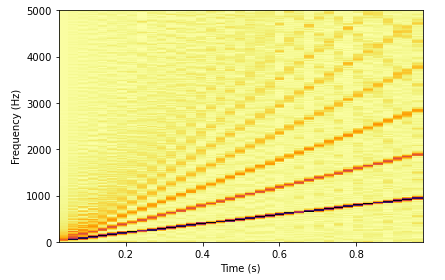
\includegraphics[width=0.75\textwidth]{2_1.png}
			\caption{Спектрограмма звука}
			\label{fig:2.1}
		\end{figure}
		
		Как видим, идет четкое повышение частоты со временем, как и в записи.
	\end{enumerate}
	
	\newpage
	
	\section{Упражнение 3.3}
	
	\begin{enumerate}
		
		\item \textbf{Задание}
		
		Создайте пилообразный чирп, меняющийся от 2500 до 3000 Гц, и на его основе сгенерируйте сигнал длительностью 1 с и частотой кадров 20 кГц. Нарисуйте, каким примерно будет \textit{Spectrum}. Затем распечатайте \textit{Spectrum} и посмотрите, правы ли вы.
		
		\item \textbf{Ход работы}
		
		Создадим пилообразный чирп и на его основе сгенерируем сигнал
		\begin{lstlisting}[caption=Чирп и сигнал]
			signal = SawtoothChirp(start=2500, end=3000)
			wave = signal.make_wave(duration=1, framerate=20000)
			wave.make_audio()
		\end{lstlisting}
		
		Получился очень острый нарастающий звук, который можно было бы использовать в каком нибудь старом советском фильме про космос.
		
		Теперь посмотрим на его спектр
		\begin{lstlisting}[caption=Создание спектра]
			wave.make_spectrum().plot()
			decorate(xlabel='Frequency (Hz)')
		\end{lstlisting}
		\begin{figure}[H]
			\centering
			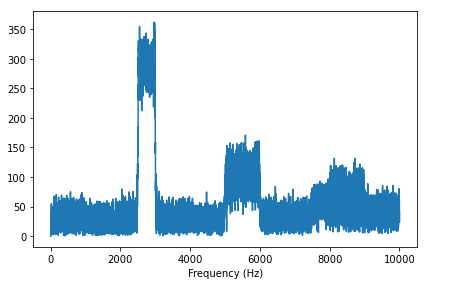
\includegraphics[width=0.75\textwidth]{3_1.png}
			\caption{Спектр}
			\label{fig:3.1}
		\end{figure}
		
		Видно, что частота отчеливо меняется, что и слышно в записи звука.
		
	\end{enumerate}
	
	\newpage
	
	\section{Упражнение 3.4}
	
	\begin{enumerate}
		
		\item \textbf{Задание}
		
		В музыкальной терминологии глиссандо - это нота, меняющаяся от одной высоты до другой, то есть своеобразный чирп.
		Найдите или запишите звук глиссандо и распечатайте спектрограмму первых нескольких секунд.
		
		
		\item \textbf{Ход работы}
		
		В выбрал фрагмент из одного из выступлений Витаса.
		\begin{lstlisting}[caption=Воспроизведение глиссандо и построение спектрограммы]
			wave = read_wave('res/vitas.wav')
			wave.make_audio()
			
			wave.make_spectrogram(512).plot(high=5000)
			decorate(xlabel='Time (s)', ylabel='Frequency (Hz)')
		\end{lstlisting}
		\begin{figure}[H]
			\centering
			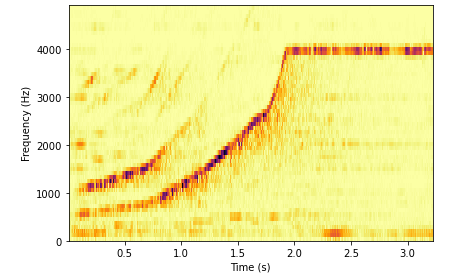
\includegraphics[width=0.75\textwidth]{4_1.png}
			\caption{Спектрограмма глиссандо}
			\label{fig:4.1}
		\end{figure}
		
		Четко видно резкое повышение частоты.
		
	\end{enumerate}
	
	\newpage
	
	\section{Упражнение 3.5}
	
	\begin{enumerate}
		
		\item \textbf{Задание}
		
		Тромбонист играет глиссандо, непрерывно дуя в мундштук и двигая кулису тромбона. При этом общая длина турбы меняется, а играемая нота обратно пропорциональна этой длине.
		
		Если предположить, что музыкант двигает кулису с постоянной скоростью, как будет меняться во времени частота?
		
		Напишите класс, называемый \textit{TromboneGliss}, расширяющий \textit{Chirp} и предоставляющий \textit{evaluate}. Создайте сигнал, имитирующий глиссандо на тромбоне от C3 до F3, и обратно до C3.
		C3 - 262 Гц
		F3 - 349 Гц
		
		Напечатайте спектрограмму полученного сигнала. На что похоже глиссандо на тромбоне - на линейный или же экспоненциальный чирп?
		
		\item \textbf{Ход работы}
		
		Напишем класс \textit{TromboneGliss}
		\begin{lstlisting}[caption=Класс \textit{TromboneGliss}]
			class TromboneGliss(Chirp):
			
			def evaluate(self, ts):
			l1, l2 = 1.0 / self.start, 1.0 / self.end
			lengths = np.linspace(l1, l2, len(ts))
			freqs = 1 / lengths
			
			dts = np.diff(ts, prepend=0)
			dphis = PI2 * freqs * dts
			phases = np.cumsum(dphis)
			ys = self.amp * np.cos(phases)
			return ys
		\end{lstlisting}
		
		Теперь создадим первую, убывающую, часть звука
		\begin{lstlisting}[caption=Создание убывающей части звука]
			low = 262
			high = 349
			signal = TromboneGliss(high, low)
			wave1 = signal.make_wave(duration=1)
			wave1.apodize()
			wave1.make_audio()
		\end{lstlisting}
		
		Теперь создадим вторую, возрастающую, часть звука
		\begin{lstlisting}[caption=Создание возрастающей части звука]
			signal = TromboneGliss(low, high)
			wave2 = signal.make_wave(duration=1)
			wave2.apodize()
			wave2.make_audio()
		\end{lstlisting}
		
		Теперь соединим две части
		\begin{lstlisting}[caption=Соединение двух частей]
			wave = wave1 | wave2
			wave.make_audio()
		\end{lstlisting}
		
		И построим спектрограмму получившегося звука
		\begin{lstlisting}[caption=Создание спектрограммы получившегося звука]
			sp = wave.make_spectrogram(1024)
			sp.plot(high=1000)
			decorate(xlabel='Time (s)', ylabel='Frequency (Hz)')
		\end{lstlisting}
		\begin{figure}[H]
			\centering
			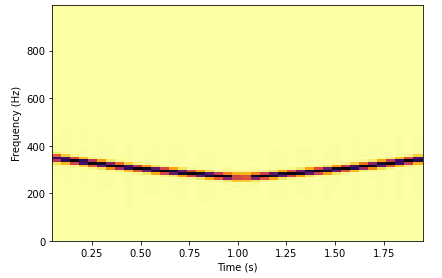
\includegraphics[width=0.75\textwidth]{5_1.png}
			\caption{Спектрограмма получившегося звука}
			\label{fig:5.1}
		\end{figure}
		
		Четко видно убывание и возрастание. Также получившийся сигнал похож на линейный чирп.
		
	\end{enumerate}
	
	\newpage
	
	\section{Упражнение 3.6}
	
	\begin{enumerate}
		
		\item \textbf{Задание}
		
		Сделайте или найдите запись серии гласных звуков и посмотрите на спектрограмму. Сможете ли вы различить разные глассные?
		
		
		\item \textbf{Ход работы}
		
		Я взял звуки из како-то детской передачи по изучению гласных. Построим спектрограмму.
		\begin{lstlisting}[caption=Построение спектрограммы гласных звуков]
			wave = read_wave('res/vowels.wav')
			wave.make_audio()
			
			wave.make_spectrogram(1024).plot(high=1000)
			decorate(xlabel='Time (s)', ylabel='Frequency (Hz)')
		\end{lstlisting}
		\begin{figure}[H]
			\centering
			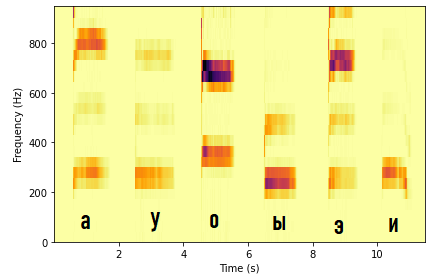
\includegraphics[width=0.75\textwidth]{6_1.png}
			\caption{Спектрограмма гласных звуков}
			\label{fig:5.1}
		\end{figure}
		
		Видно, что участки некоторых глассных темнее, а некоторых - светлее.
		
		Посмотрим на спектры каждой гласной.
		\begin{lstlisting}[caption=Спектр буквы а]
			high = 1000
			
			segment = wave.segment(start=0, duration=2)
			segment.make_spectrum().plot(high=high)
		\end{lstlisting}
		\begin{figure}[H]
			\centering
			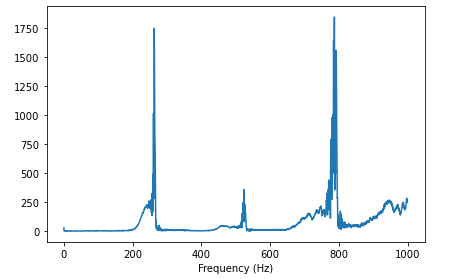
\includegraphics[width=0.75\textwidth]{6_2.png}
			\caption{Спектр буквы а}
			\label{fig:6.2}
		\end{figure}
		
		\begin{lstlisting}[caption=Спектр буквы у]
			segment = wave.segment(start=2, duration=2)
			segment.make_spectrum().plot(high=high)
			decorate(xlabel='Frequency (Hz)')
		\end{lstlisting}
		\begin{figure}[H]
			\centering
			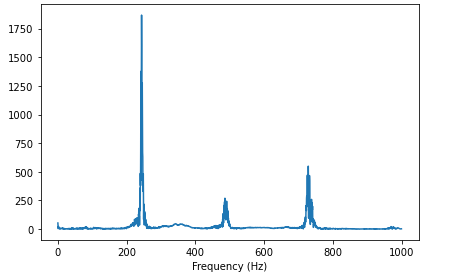
\includegraphics[width=0.75\textwidth]{6_3.png}
			\caption{Спектр буквы у}
			\label{fig:6.3}
		\end{figure}
		
		\begin{lstlisting}[caption=Спектр буквы о]
			segment = wave.segment(start=4, duration=2)
			segment.make_spectrum().plot(high=high)
			decorate(xlabel='Frequency (Hz)')
		\end{lstlisting}
		\begin{figure}[H]
			\centering
			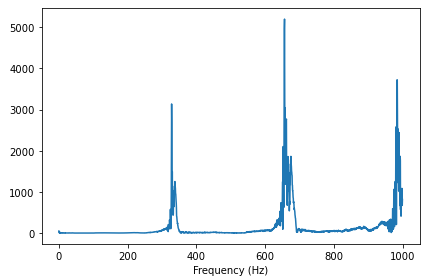
\includegraphics[width=0.75\textwidth]{6_4.png}
			\caption{Спектр буквы о}
			\label{fig:6.4}
		\end{figure}
		
		\begin{lstlisting}[caption=Спектр буквы ы]
			segment = wave.segment(start=6, duration=2)
			segment.make_spectrum().plot(high=high)
			decorate(xlabel='Frequency (Hz)')
		\end{lstlisting}
		\begin{figure}[H]
			\centering
			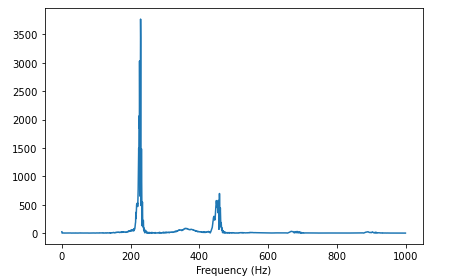
\includegraphics[width=0.75\textwidth]{6_5.png}
			\caption{Спектр буквы ы}
			\label{fig:6.5}
		\end{figure}
		
		\begin{lstlisting}[caption=Спектр буквы э]
			segment = wave.segment(start=8, duration=2)
			segment.make_spectrum().plot(high=high)
			decorate(xlabel='Frequency (Hz)')
		\end{lstlisting}
		\begin{figure}[H]
			\centering
			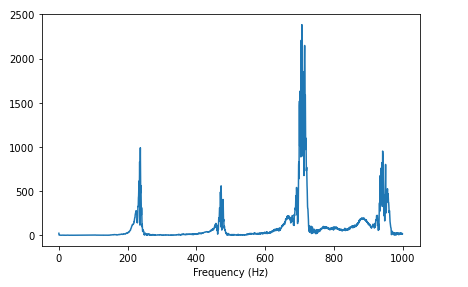
\includegraphics[width=0.75\textwidth]{6_6.png}
			\caption{Спектр буквы э}
			\label{fig:6.6}
		\end{figure}
		
		\begin{lstlisting}[caption=Спектр буквы и]
			segment = wave.segment(start=10, duration=2)
			segment.make_spectrum().plot(high=high)
			decorate(xlabel='Frequency (Hz)')
		\end{lstlisting}
		\begin{figure}[H]
			\centering
			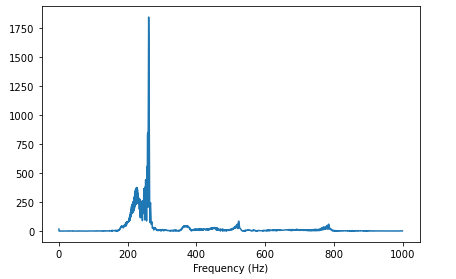
\includegraphics[width=0.75\textwidth]{6_7.png}
			\caption{Спектр буквы и}
			\label{fig:6.7}
		\end{figure}
		
		
		Из графиков видно, что спектр каждой гласной имеет разную высоту. 
		Чем выше спектр, тем темнее спектрограмма.
		
		
	\end{enumerate}
	
	\newpage
	
	\section{Вывод}
	
	В результате выполнения лабораторной работы получены навыки работы с апериодическими сигналами - сигналами, частотные компоненты которых изменяются во времени, чирпами - сигналами с переменной частотой. Также получены навыки построения спектрограмм и их анализ.
	
\end{document}